\documentclass[border=6pt]{standalone}
\usepackage{tikz}
\usetikzlibrary{arrows.meta,positioning,calc,shapes.geometric,fit,backgrounds,patterns,matrix,decorations.pathreplacing}
\begin{document}
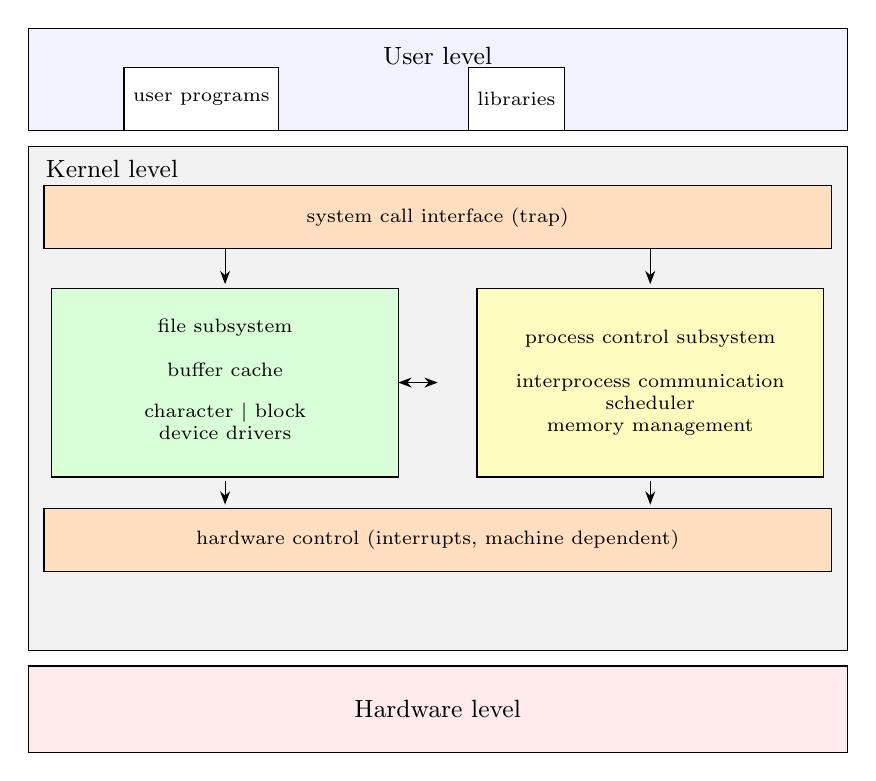
\begin{tikzpicture}[>=Stealth,font=\small]
\tikzstyle{b}=[draw,align=center,font=\scriptsize,minimum height=0.8cm]
\draw[fill=blue!5] (-0.2,6.6) rectangle (10.2,7.9); \node[font=\small] at (5,7.55) {User level};
\node[b,fill=white] at (2,7.0) {user programs}; \node[b,fill=white] at (6,7.0) {libraries};
\draw[fill=gray!10] (-0.2,0) rectangle (10.2,6.4);
\node[font=\small,anchor=north west] at (-0.1,6.35) {Kernel level};
\node[b,fill=orange!25,minimum width=10cm] at (5,5.5) {system call interface (trap)};
\node[b,fill=green!15,minimum width=4.4cm,minimum height=2.4cm] at (2.3,3.4) {file subsystem\\ \\ buffer cache\\ \\ \begin{tabular}{@{}c@{}}character $|$ block\\ device drivers\end{tabular}};
\node[b,fill=yellow!25,minimum width=4.4cm,minimum height=2.4cm] at (7.7,3.4) {process control subsystem\\ \\ interprocess communication\\ scheduler\\ memory management};
\draw[->] (2.3,5.1) -- (2.3,4.65); \draw[->] (7.7,5.1) -- (7.7,4.65);
\draw[<->] (5,3.4) -- (4.5,3.4);
\node[b,fill=orange!25,minimum width=10cm] at (5,1.4) {hardware control (interrupts, machine dependent)};
\draw[->] (2.3,2.15) -- (2.3,1.85); \draw[->] (7.7,2.15) -- (7.7,1.85);
\draw[fill=red!8] (-0.2,-1.3) rectangle (10.2,-0.2); \node[font=\small] at (5,-0.75) {Hardware level};
\end{tikzpicture}
\end{document}
